\chapter{Simulado 1}

Leia o cartaz de uma campanha publicitária para responder às questões de
1 a 5.

%\textbf{http://agenciaal.alesc.sc.gov.br/index.php/sala\_imprensa\_single/novas-pecas-publicitarias-daeo-desfecho-a-campanha-adocaeo-lacos-de-amor\#!prettyPhoto}

\begin{figure}
\centering
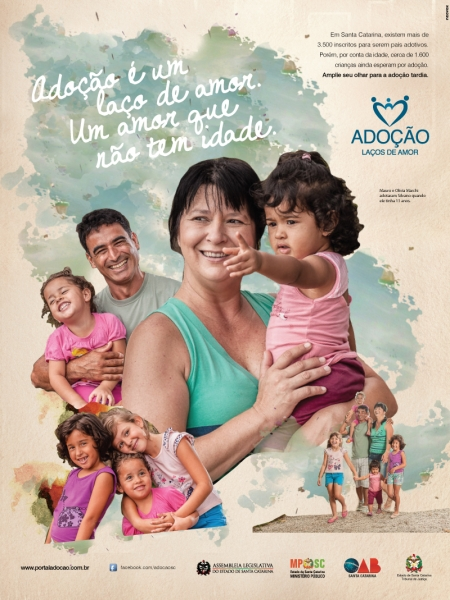
\includegraphics[width=4.68750in,height=6.25000in]{./_SAEB_9_POR/media/image33.jpeg}
\end{figure}

%\textbf{Disponível em: \textless{}http://agenciaal.alesc.sc.gov.br/index.php/sala\_imprensa\_single/novas-pecas-publicitarias-daeo-desfecho-a-campanha-adocaeo-lacos-de-amor\#!prettyPhoto\textgreater{}. Acesso em: 9 abr. 2023.}

\num{1} O público-alvo dessa campanha são

\begin{escolha}
  crianças que estão na fila de espera da adoção.
\item
  pessoas que desejam participar do processo de adoção.
\item
  famílias que querem entregar uma criança para a adoção.
\item
  cidadãos que já adotaram crianças.
\end{enumerate}


\num{2} Mais especificamente, que tipo de processo de adoção é estimulado por
meio da expressão ``um amor que não tem idade''?

\begin{escolha}
  adoção por parte de pais jovens.
\item
  adoção para crianças que ainda não nasceram.
\item
  adoção de crianças crescidas, que já não são bebês.
\item
  adoção de irmãos.
\end{enumerate}


\num{3} Como as imagens e o texto verbal dialogam nesse anúncio?

\begin{escolha}
  imagem e texto verbal geram incoerência proposital, para chamar a
  atenção dos leitores.
\item
  imagem e texto verbal se contradizem, invalidando a mensagem trazida
  pelo anúncio.
\item
  texto verbal e texto não verbal não se relacionam diretamente.
\item
  texto verbal e imagem se complementam, sendo o anúncio um texto
  multissemiótico.
\end{enumerate}


\num{4} O anúncio é do estado de Santa Catarina, o que se comprova

\begin{escolha}
  pelo texto verbal em letras menores, no alto, à direita.
\item
  pelas imagens apresentadas, que mostram características geográficas do
  estado.
\item
  pelo slogan que, como qualquer brasileiro pode notar, remete ao
  estado.
\item
  pelo texto maior, em letras brancas, que parece manuscrito.
\end{enumerate}

\num{5} Na parte inferior do cartaz, em miniatura, aparecem

\begin{escolha}
  brasões de famílias que passaram pelo processo de adoção.
\item
  símbolos de órgãos que apoiam a campanha.
\item
  símbolos de instituições que acolhem crianças.
\item
  marcas de empresas que financiam processos de adoção.
\end{enumerate}

Leia um trecho do texto acerca da construção dos espetáculos teatrais.
Depois, responda às questões 6 e 7.

\begin{quote}
\textbf{Corpo, Expressão e Movimento}

{[}\ldots{}{]} Você sabe como acontece a construção de uma peça teatral?

%Imagem ilustrativa que pode ser cortada: \url{https://www.freepik.com/free-photo/mime-reading-manuscript-stage-empty-auditorium_2975761.htm\#query=theatre\&position=29\&from_view=search\&track=sph}

O processo de criação teatral envolve todo um coletivo em pesquisa,
jogos teatrais e improvisação. Ele pode ser feito por meio de um texto
pré-existente ou mesmo na construção de um novo texto. Assim vão se
definindo personagens, cenas e outros elementos que compõem o espetáculo
teatral.

\fonte{CORPO, expressão e movimento. Disponível em:
http://sme.goiania.go.gov.br/conexaoescola/eaja/musica-e-teatro/. Acesso
em: 9 abr. 2023.}
\end{quote}

\num{6} Pela leitura do texto, pode-se afirmar que os jogos teatrais e a
improvisação

\begin{escolha}
\item representam o resultado final da encenação e são sempre reproduzidos
da mesma forma.

\item mostram como é a forma correta de se representar uma cena teatral a
partir de um texto.

\item são parte da preparação da peça, pois auxiliam no processo de
construção do espetáculo.

\item fazem parte de um processo utilizado pelos atores, porque eles
dependem da presença de plateia.
\end{escolha}

\num{7} A pergunta presente no título do texto

\begin{escolha}
\item mostra que não haverá respostas, elas devem ser buscadas pelo
leitor.

\item apresenta, em si mesma, um passo a passo para a construção da peça
teatral.

\item aponta para o fato de que haverá muitos dados estatísticos no texto.

\item dirige-se diretamente ao leitor, gerando nele curiosidade e vontade
de ler o texto.
\end{escolha}

\num{8} Leia o texto.

\begin{quote}
Foi um renomado pintor norueguês do final do século XIX e início do século XX. 
Ele é conhecido por ser um dos pioneiros do movimento expressionista. Sua obra 
mais famosa é ``O grito'', que retrata angústia e desespero. Munch explorou temas 
como a mortalidade e a fragilidade humana em suas pinturas. Sua contribuição para 
a arte moderna foi significativa e suas obras continuam a cativar pessoas ao redor 
do mundo. Ele faleceu em 1944, deixando um legado duradouro na história da arte.

\fonte{Texto escrito para este material.}
\end{quote}

O artista descrito no texto é

\begin{escolha}
\item
  Vincent van Gogh.
\item
  Ernst Kirchner.
\item
  Edvard Munch.
\item
  Wassily Kandinsky.
\end{escolha}




\num{9} Observe a pintura.

\begin{figure}[htpb!]
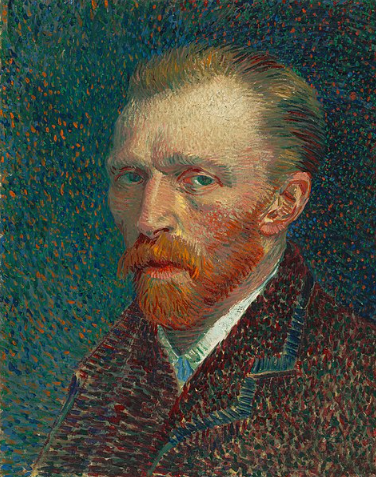
\includegraphics[width=3.16667in,height=4.01042in]{media/image28.png}
\caption{Óleo sobre tela de Vincent van Gogh, de 1887}
\end{figure}

%https://commons.wikimedia.org/wiki/File:Vincent\_van\_Gogh\_-\_Self-Portrait\_-\_Google\_Art\_Project\_(454045).jpg\textgreater{}


Essa pintura pertence ao gênero

\begin{escolha}
\item
  autorretrato.
\item
  natureza-morta.
\item
  paisagem.
\item
  retrato.
\end{escolha}


\num{10} Leia o texto.

\begin{quote}
A instalação \emph{Ambiente -- Sala de jantar} expõe entre paredes de
\textit{nylon} pinturas, com \textit{spray} azul, de objetos e móveis. No espaço interno,
encontra-se uma mesa posta com pratos de louça, copos de vidro, garfos e
facas em inox, associada a uma gravação de áudio com as sonoridades
próprias de uma refeição: diálogo entre pessoas e ruído de talheres e
pratos. O foco de luz incide sobre a mesa.

\fonte{Texto escrito para este material.}
\end{quote}

A escolha do tema descrito no texto permitiu que a
artista portuguesa Ana Vieira integrasse diferentes linguagens
artísticas. Assinale a alternativa que contém duas fontes materiais
utilizadas na obra.

\begin{escolha}
\item
  Espaço e gesto.
\item
  Instrumento musical e tinta \textit{spray}.
\item
  Luz e som.
\item
  Pincel e som.
\end{escolha}

\num{11} Leia o texto.

\begin{quote}
\textbf{NASA-funded Research Reveals Alarming Risk of Antarctic Ice
Sheets Melting}

There are numerous ominous signs of the repercussions of climate change,
but few cause more concern for scientists than the ice sheets in
Antarctica, located at the southern pole of our planet. These ice sheets
have been melting for a considerable period of time, and it doesn't
require an advanced degree in physics to comprehend the risks involved.
As the ice thaws, it flows into the ocean, causing sea levels to rise,
which is an obvious and significant problem.

A new study published in the journal PNAS, which was funded by NASA,
reveals an alarming complication. Scientists from the Georgia Institute
of Technology, NASA Jet Propulsion Laboratory, and the University of
Washington conducted hundreds of simulations to predict how one massive
ice sheet, Thwaites Glacier, could deteriorate over the next 50 to 800
years. The findings indicated that the glacier is more prone to
instability than was previously assumed.

\fonte{Fonte de pesquisa: A. J. Willingham. CNN. Antarctica’s ice is degrading faster than we thought, and there may be no way to stop the consequences. Disponível em: *https://edition.cnn.com/2019/07/10/world/antarctica-ice-sheet-sea-levels-trnd/index.html*. Acesso em: 01 mar. 2023.}
\end{quote}

O texto reproduzido trata

\begin{escolha}
\item das consequências das mudanças climáticas no Brasil.

\item de formas de impedirmos o derretimento do gelo na Antártica.

\item do ritmo de derretimento do gelo antártico.

\item da ameaça aos animais da Antártida.
\end{escolha}

\num{12} Leia o texto.

\begin{quote}
\textbf{Climate Change Study Warns of Severe Droughts in London by 2050}

A new climate change study states that by 2050, London's climate will
resemble that of Barcelona. However, this doesn't imply a pleasant
warming. In fact, London might confront severe droughts, as Barcelona
did in 2008 when it almost depleted its drinking water and reservoirs
came close to drying out.

The study conducted by the Crowther Lab at ETH Zurich university reveals
that hundreds of other major cities worldwide may also face droughts,
floods, storms, and other climate catastrophes.

\fonte{Fonte de pesquisa: Jessie Yeung. CNN. By 2050,
London's climate will be as warm as Barcelona's, says new study.
Disponível em:
\emph{https://edition.cnn.com/2019/07/11/europe/climate-cities-report-intl-hnk/index.html}.
Acesso em: 01 mar. 2023.}
\end{quote}

De acordo com o texto, o aumento das temperaturas na Inglaterra terá
como consequência

\begin{escolha}
\item a diminuição de tempestades em Londres.

\item o aumento do nível dos rios em Londres.

\item uma seca severa em Barcelona.

\item uma seca severa em Londres.
\end{escolha}

\num{13} Leia o texto.

\begin{quote}
\textbf{Dracula}

Just before I was leaving, the old lady came up to my room and said in a
very hysterical way:

``Must you go? Oh! young Herr, must you go?'' She was in such an excited
state that she seemed to have lost her grip of what German she knew, and
mixed it all up with some other language which I did not know at all. I
was just able to follow her by asking many questions {[}\ldots{}{]}.

\fonte{Bram Stoker. \emph{Dracula}. Disponível em:
\emph{https://www.gutenberg.org/cache/epub/345/pg345-images.html}.
Acesso em: 01 mar. 2023.}
\end{quote}

Esse trecho faz parte de um texto

\begin{escolha}
\item literário.

\item argumentativo.

\item noticioso.

\item instrucional.
\end{escolha}

\num{14} Leia o texto.

\begin{quote}
Carvão é o nome dado a diversas rochas sedimentares passíveis
de uso como combustível, constituídas de um material heterogêneo
originado de restos vegetais depositados em águas rasas, protegidos da
ação do oxigênio do ar. {[}...{]}

A extração do carvão pode ser em minas a céu aberto ou
subterrâneas, dependendo da profundidade em que se encontra a camada. As
minas a céu aberto exercem significativo impacto ambiental em razão dos
elementos químicos contidos no carvão, como o enxofre.

Numerosas áreas de mineração antigas no sul do Brasil, trabalhadas
em uma época em que a preocupação com o ambiente natural era muito menor
que atualmente, foram muito degradadas e precisaram ser recuperadas,
trabalho que vem sendo feito nas últimas décadas.

{[}...{]}

\fonte{Serviço Geológico do Brasil. Carvão mineral. Disponível em:
\emph{http://www.cprm.gov.br/publique/SGB-Divulga/Canal-Escola/Carvao-Mineral-2558.html}.
Acesso em: 28 fev. 2023.}
\end{quote}

É possível identificar que o principal impacto da extração de carvão se dá pela

\begin{escolha}
\item
  emissão local de fumaça.
\item
  geração de ilhas de calor.
\item
  exaustão do lençol freático.
\item
  remoção da estrutura superficial do solo.
\end{escolha}

\num{15} Analise o esquema.

%\begin{figure}[htpb!]
%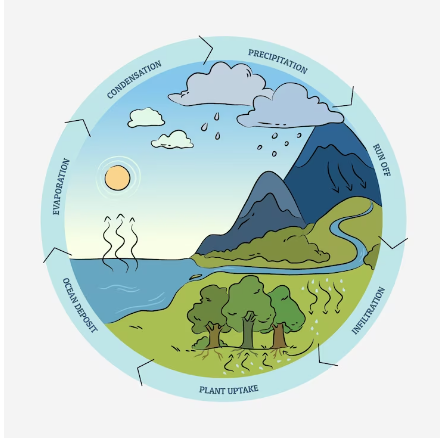
\includegraphics[width=4.58333in,height=4.56250in]{./imgs/img9.png}
%\caption{Fonte:
%https://br.freepik.com/vetores-gratis/informacoes-desenhadas-a-mao-sobre-o-ciclo-da-agua\_18980469.htm\#query=ciclo\%20da\%20agua\&position=1\&from\_view=keyword\&track=ais.}
%\end{figure}
%Paulo, trocar foto: https://br.freepik.com/vetores-gratis/desenho-a-mao-de-um-ciclo-de-agua-de-design-plano_18773933.htm#query=informacoes%20desenhadas%20a%20mao%20sobre%20o%20ciclo%20da%20agua&position=2&from_view=search&track=ais

No ciclo da água, a absorção de energia ocorre

\begin{escolha}
\item
  no escoamento.
\item
  na precipitação.
\item
  na condensação.
\item
  na evaporação.
\end{escolha}

\num{16} Leia o texto.

\begin{quote}
\textbf{Capacidade de geração de energia eólica deve bater recorde neste ano}

O Brasil registra, até fevereiro [de 2023], 890 parques eólicos instalados em 12 estados brasileiros. Eles somam 25,04 gigawatts (GW) de capacidade instalada em operação comercial, que beneficiam 108,7 milhões de habitantes.

Desse total, 85\% estão na Região Nordeste. De acordo com a Associação Brasileira de Energia Eólica (Abeeólica), até 2028 o Brasil terá 44,78 GW de capacidade instalada desse tipo de energia, cuja participação na matriz nacional atinge, atualmente, 13,2\%. A eólica já responde hoje por 20\% da geração de energia [de] que o país precisa.

No ano passado, o setor bateu recorde de 4 GW instalados e, para este ano, a presidente executiva da Abeeólica, Elbia Gannoum, espera atingir novo recorde, superando esse número. “Encerrando 2023, estaremos com 29 GW de capacidade instalada. Essa é a nossa previsão em termos de potência, e isso é superior a R\$ 28 bilhões, porque cada gigawatt de eólica instalada é da ordem de R\$ 7 bilhões”, disse Elbia {[}...{]}.

\fonte{Alana Gandra. Agência Brasil. Capacidade de geração de energia eólica deve bater recorde neste ano. Disponível em:
\emph{https://agenciabrasil.ebc.com.br/economia/noticia/2023-04/capacidade-de-geracao-de-energia-eolica-deve-bater-recorde-neste-ano}.
Acesso em: 05 abr. 2023.}
\end{quote}

O texto demonstra que o Brasil

\begin{escolha}
\item
  está avançando na produção de energia de uma fonte renovável.
\item
  é dependente de um tipo de energia que não tem muito potencial no país.
\item
  produz mais energia eólica do que a de qualquer outro tipo.
\item
  tem aumentado a produção de energia de fonte não renovável.
\end{escolha}

\num{17} Leia o texto.

\begin{quote}
\textbf{Cota racial}

Em vigor desde 10 de junho de 2014, a Lei 12.990 prevê uma cota de vagas para negros e pardos em concursos públicos, com o objetivo de reduzir as desigualdades sociais, econômicas e educacionais entre as raças e promover uma maior inclusão e diversidade nos cargos públicos.

\fonte{Jusbrasil. Entenda como funciona a "cota racial" para concursos públicos no Brasil. Disponível em: \emph{https://www.jusbrasil.com.br/artigos/entenda-como-funciona-a-cota-racial-para-concursos-publicos-no-brasil/243608268}. Acesso em: 04 maio 2023.}
\end{quote}

Tal como em vestibulares, as cotas nos concursos públicos buscam

\begin{escolha}
\item  discriminar racialmente a população branca.

\item  conferir privilégios para minorias demográficas.

\item  compor uma política ampla de reparação histórica.

\item  estabelecer mecanismos de compensação para incapazes.
\end{escolha}


\num{18} Leia o texto.

\begin{quote}
\textbf{ONGs apontam racismo em falta de políticas públicas em áreas de risco}

A falta de políticas públicas voltadas a atender à demanda da população negra e periférica que vive em áreas de risco ambiental –-- como nos locais atingidos por deslizamentos de terra no litoral Norte de São Paulo --- é uma opção das administrações públicas e demonstra racismo ambiental. A avaliação é de especialistas de duas organizações da sociedade civil, o Greenpeace e o Instituto Polis.

``[O racismo ambiental] está muito ligado à segregação e [à] exclusão em relação ao direito de ter o meio ambiente de determinada região equilibrado. A gente observa a escolha política, o critério para definir locais que vão ter políticas públicas. E elas não conseguem chegar sempre à população dos morros, negra e periférica'', afirma Rodrigo Jesus, da Campanha Clima e Justiça, do Greenpeace.

De acordo com ele, a falta de prioridade das populações negra e periférica demonstra ainda negligência. {[}...{]}

\fonte{Bruno Bocchini. Agência Brasil. ONGs apontam racismo em falta de políticas públicas em áreas de risco. Disponível em: \emph{https://agenciabrasil.ebc.com.br/geral/noticia/2023-02/ongs-apontam-racismo-em-falta-de-politicas-publicas-em-areas-de-risco}. Acesso em: 04 maio 2023.}
\end{quote}

A criação de canais de representação e participação popular da população
negra contribuiria para a diminuição de desastres ambientais de maneira
geral ao

\begin{escolha}
\item  organizar os governos locais.

\item  valorizar pautas esquecidas no debate público.

\item  explicar os mecanismos dos desastres ambientais.

\item  adequar o orçamento dirigido a obras públicas pontuais.
\end{escolha}